\documentclass[12pt]{article}
\usepackage[utf8]{inputenc}
\usepackage{graphicx}
\usepackage{amsmath}
\usepackage[margin=1in]{geometry}
\usepackage{indentfirst}
\usepackage{amsfonts}
%for english
\usepackage[portuguese]{babel}
%for portuguese
%\usepackage[portuguese]{babel}
\usepackage{float}
\usepackage[usenames,dvipsnames]{color}

\usepackage{listings}
\usepackage{color}

\definecolor{mygreen}{rgb}{0,0.6,0}
\definecolor{mygray}{rgb}{0.5,0.5,0.5}
\definecolor{mymauve}{rgb}{0.58,0,0.82}


\lstset{ %
  backgroundcolor=\color{white},   % choose the background color; you must add \usepackage{color} or \usepackage{xcolor}
  basicstyle=\footnotesize,        % the size of the fonts that are used for the code
  breakatwhitespace=false,         % sets if automatic breaks should only happen at whitespace
  breaklines=true,                 % sets automatic line breaking
  captionpos=b,                    % sets the caption-position to bottom
  commentstyle=\color{mygreen},    % comment style
  deletekeywords={...},            % if you want to delete keywords from the given language
  escapeinside={\%*}{*)},          % if you want to add LaTeX within your code
  extendedchars=true,              % lets you use non-ASCII characters; for 8-bits encodings only, does not work with UTF-8
  frame=single,                    % adds a frame around the code
  keepspaces=true,                 % keeps spaces in text, useful for keeping indentation of code (possibly needs columns=flexible)
  keywordstyle=\color{blue},       % keyword style
  language=C,                 % the language of the code
  morekeywords={*,...},            % if you want to add more keywords to the set
  numbers=left,                    % where to put the line-numbers; possible values are (none, left, right)
  numbersep=5pt,                   % how far the line-numbers are from the code
  numberstyle=\tiny\color{mygray}, % the style that is used for the line-numbers
  rulecolor=\color{black},         % if not set, the frame-color may be changed on line-breaks within not-black text (e.g. comments (green here))
  showspaces=false,                % show spaces everywhere adding particular underscores; it overrides 'showstringspaces'
  showstringspaces=false,          % underline spaces within strings only
  showtabs=false,                  % show tabs within strings adding particular underscores
  stepnumber=1,                    % the step between two line-numbers. If it's 1, each line will be numbered
  stringstyle=\color{mymauve},     % string literal style
  tabsize=2,                       % sets default tabsize to 2 spaces
  title=\lstname                   % show the filename of files included with \lstinputlisting; also try caption instead of title
}




\begin{document}
\renewcommand*\contentsname{Índice}

\begin{titlepage}

\newcommand{\HRule}{\rule{\linewidth}{0.5mm}} 
\center 
 

\textsc{\LARGE Universidade de Coimbra}\\[1.5cm] % Name of your university/college
\textsc{\Large Departamento de Engenharia Informática}\\[4cm] % Major heading such as course name
\textsc{\large Compiladores 2013/2014}\\[1cm] % Minor heading such as course title


\HRule \\[0.5cm]
{ \huge \bfseries Compilador para linguagem iJava}\\[0.4cm] 
\HRule \\[8cm]
 
\begin{minipage}{0.4\textwidth}
\begin{flushleft} \large
\emph{Autor:}\\
David \textsc{Cardoso}  \\Número: 2011164039
\end{flushleft}
\end{minipage}
~
\begin{minipage}{0.4\textwidth}
\begin{flushright} \large
\emph{Autor:} \\
Bruno \textsc{Caceiro}  \\Número: 2008107991
\end{flushright}
\end{minipage}\\[2cm]

{\large \today}\\[3cm]

\vfill

\end{titlepage}


\tableofcontents
\vfill
\pagebreak


\section{Introdução}
Este projecto consiste no desenvolvimento de um compilador para a linguagem \emph{iJava} (imperative Java), que consiste num pequeno subconjunto da linguagem Java (versão 5.0). Os programas da linguagem \emph{iJava} são constituídos por uma única classe (a principal), contendo necessariamente um método \emph{main}, e podendo conter outros métodos e atributos, todos eles estáticos e (possivelmente) públicos.

O projecto foi estruturado em 3 fases, primeiramente foi feita a Análise Lexical, implementada na linguagem \emph{C} e utilizando a ferramenta \emph{lex}. A segunda fase consistiu na análise sintática, com a  construção da árvore de sintaxe abstrata e análise semântica (tabelas de símbolos, deteção de erros semânticos). No final foi feita a geração de código.

\begin{figure}[H]
       \centering
       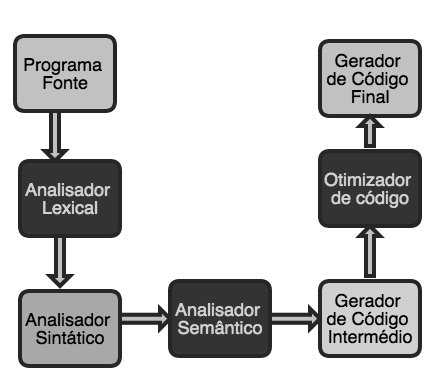
\includegraphics[keepaspectratio=true, width=300px]{fasesCompilacao.png}
       \caption{Fases de Compilação}
       \end{figure}

\pagebreak
\section{Análise Lexical}

A Análise Lexical consiste em analisar a entrada de linhas de caracteres e produzir uma sequência de símbolos (\emph{tokens}) que podem ser manipulados mais facilmente por um \emph{parser}. É uma forma de verificar um determinado alfabeto, neste caso o alfabeto da linguagem \emph{iJava}.
Esta análise pode ser dividida em três fases:
\begin{itemize}
	\item Extração e classificação de \emph{tokens};
	\item Eliminação de delimitadores e comentários;
	\item Tratamento de erros;
\end{itemize}


\subsection{Tokens}
\begin{itemize}
	        \item \textbf{ID:} Sequências alfanuméricas começadas por uma letra, onde os símbolos "\_" e "\$" contam como letras. Maiúsculas e minúsculas são consideradas letras diferentes
	        \begin{itemize}
				\item \textbf{Expressão Regular}: $[a-zA-Z\_\$]([a-zA-Z\_\$0-9])* $
	        \end{itemize}
	         
	        \item \textbf{INTLIT:} Sequências de dígitos decimais e sequências de dígitos hexadecimais (incluindo a-f e A-F) precedidas de "0x"
	        \begin{itemize}
	        	\item \textbf{Expressão Regular:}  $(([0-9])+|("0x"[0-9a-$f$A-F]+))$  
	        \end{itemize}
	        \item \textbf{BOOLLIT:} "true" \text{\textbar} "false" 
	        \item \textbf{INT:} "int"
	        \item \textbf{BOOL:} "boolean"
	        \item \textbf{NEW:} "new"
	        \item \textbf{IF:} "if"
	        \item \textbf{ELSE:} "else"
	        \item \textbf{WHILE:} "while"
	        \item \textbf{PRINT:} "System.out.println"
	        \item \textbf{PARSEINT:} "Integer.parseInt"
	        \item \textbf{CLASS:} "class"
	        \item \textbf{PUBLIC:} "public"
	        \item \textbf{STATIC:} "static"
	        \item \textbf{VOID:} "void"
	        \item \textbf{STRING:} "String"
	        \item \textbf{DOTLENGTH:} ".length"
	        \item \textbf{RETURN:} "return"
	        \item \textbf{OCURV:} "("
	        \item \textbf{CCURV:} ")"
	        \item \textbf{OBRACE} "\{"
	        \item \textbf{CBRACE:} "\}"
	        \item \textbf{OSQUARE:} "["
	        \item \textbf{CSQUARE:} "]"	 
	        \item \textbf{ASSIGN:} "="
	        \item \textbf{SEMIC:} ";"
	        \item \textbf{COMMA:} ","
	      \end{itemize}
	      
	    Foi necessário separar alguns \emph{tokens} devido às diferentes prioridades que cada operador tem.
		\begin{itemize}  
	        \item \textbf{OP1:} "\&\&"  
	        \item \textbf{OP1OR:} "\text{\textbar} \text{\textbar}"
	        \item \textbf{OP2:} "\textless" \text{\textbar} "\textgreater" \text{\textbar} "\textless=" \text{\textbar} "\textgreater="
	        \item \textbf{OP2EQS:} "==" \text{\textbar} "!="	        
	        \item \textbf{OP3:} "+" \text{\textbar} "-"
	        \item \textbf{OP4:} "*" \text{\textbar} "/" \text{\textbar} "\%"
	        \item \textbf{NOT:} "!"
	        \end{itemize}
	         O \emph{iJava} é um subconjunto da linguagem \emph{Java}, como tal, existe um conjunto de funcionalidades que embora não sejam suportadas, têm de ser consideradas. Assim, foi necessário tratar todo um conjunto de palavras reservadas de forma a permitir que sejam lexicalmente válidas mas não sintaticamente.
	         \begin{itemize} 
	        \item \textbf{RESERVED:}
	       	            \begin{itemize}
	       	                \item abstract
	       	                \text{\textbar} assert 
	       	                \text{\textbar} break 
	       	                \text{\textbar} byte 
	       	                \text{\textbar} case 
	       	                \text{\textbar} catch 
	       	                \text{\textbar} char 
	       	                \text{\textbar} const 
	       	                \text{\textbar} continue
	       	                 \text{\textbar} default 
	       	                 \text{\textbar} do 
	       	                 \text{\textbar} double
	       	                 \text{\textbar} enum 
	       	                 \text{\textbar} extends 
	       	                 \text{\textbar} final 
	       	                 \text{\textbar} finally 
	       	                 \text{\textbar} float 
	       	                 \text{\textbar} for 
	       	                 \text{\textbar} goto 
	       	                 \text{\textbar} implements 
	       	                 \text{\textbar} import 
	       	                 \text{\textbar} instanceof
	       	                 \text{\textbar} interface 
	       	                 \text{\textbar} long
	       	                 \text{\textbar} native
	       	                 \text{\textbar} package
	       	                 \text{\textbar} private 
	       	                 \text{\textbar} protected 
	       	                 \text{\textbar} short 
	       	                 \text{\textbar} strictfp
	       	                 \text{\textbar} super 
	       	                 \text{\textbar} switch 
	       	                 \text{\textbar} synchronized 
	       	                 \text{\textbar} this 
	       	                 \text{\textbar} throw 
	       	                 \text{\textbar} throws 
	       	                 \text{\textbar} transient 
	       	                 \text{\textbar} try
	       	                 \text{\textbar} volatile
		       	             \text{\textbar} null
	       	                 \text{\textbar} ++
	       	                 \text{\textbar} --
	       	            \end{itemize}      	 
		\end{itemize}
		
		\subsubsection{Comentários}
		Existem duas maneiras de fazer comentários:
		\begin{itemize}
			\item Comentar apenas uma linha //\textless código\textgreater. \\Caso seja detectado (//)  todo o código que se segue é ignorado até encontrar uma mudança de linha.
			\subitem \textbf{Expressão Regular:} "//".*
			\item Comentar um bloco de código  /*\textless código\textgreater */
		\end{itemize} 
		\lstset{language=C,caption={Detecção de Comentários},label=Estruturas,frame=single}
		\begin{lstlisting}
		< COMMENT > <<EOF>> {BEGIN 0}
		< COMMENT > "*/"    {BEGIN 0}
		< COMMENT > "\n"    {}
		< COMMENT > .       {}
		"/*"	            {BEGIN COMMENT}
		\end{lstlisting}
		Caso seja detectado (/*) todo o código é ignorado até que seja encontrado o seu correspondente (*/). Caso seja detectado o EOF então é apresentada uma mensagem de erro: "Line \%d, col \%d: unterminated comment". Foi criado um estado adicional no \emph{lex} para poder esta situação.
		
		
		
		\subsubsection{Tratamento de Erros}
		Se forem detectados erros lexicais no ficheiro de entrada então é impressa uma mensagem de erro no \emph{stdout}:
		\begin{itemize}
            \item "Line\textless num linha\textgreater,col\textless num coluna\textgreater:illegal character('\textless c \textgreater'\textbackslash n)"
            \item "Line\textless num linha\textgreater,col\textless num coluna\textgreater:unterminated comment\textbackslash n"
        \end{itemize}
        Para podermos imprimir as mensagens de erro com o número da linha e coluna criámos uma variável \emph{column} para poder contar as colunas e utilizamos a variável \emph{yylineno} disponibilizada pelo \emph{yacc} para sabermos o número das linhas.
        Para a contagem de colunas aumentamos a variável referente às colunas consoante o tamanho de cada \emph{token}. Quando há uma mudança de linha, inicializa-se o contador das colunas a 1. \\Para tratar o caso dos comentários criámos duas variáveis adicionais (\emph{Commentline,Commentcolumn}) para poder guardar a coluna e linha onde o comentário é inicializado.
        
	
\pagebreak

\section{Análise Sintática e Semântica}
O \emph{lex} vai reconhecer os \emph{tokens} para de seguida o \emph{yacc} verificar se estes pertencem à gramática da linguagem.


\begin{figure}[H]
       \centering
       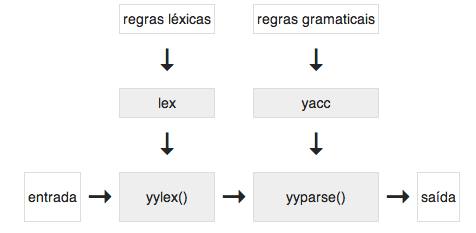
\includegraphics[keepaspectratio=true, scale = 0.82]{lex_yacc.png}
       \caption{Relacionamento entre \emph{lex} e \emph{yacc}, retirado de \emph{http://pt.wikipedia.org/wiki/Yacc}}
       \end{figure}
       
Para realizar a ligação entre o yacc e o lex foram definimos tokens no  yacc ,posteriormente importados pelo lex. Sempre que o lex uma sequência de caracteres correspondente a um token válido retorna-o, sendo este valor enviado para o yacc.     
\par É a variável \emph{yylval} que contém tipicamente o valor do \emph{token} encontrado num dado momento. Uma vez que pretendemos enviar vários de dados, tivémos e utilizar uma \emph{union}, definida no \emph{yacc},que permite partilhar, no mesmo espaço de memória, vários tipos diferentes.
\lstset{language=c,caption={Union},label=Estruturas}
\begin{lstlisting}
%union{
    struct _Node* node;
    char* token;
    struct _idList* listId;
    int type;
}
\end{lstlisting}       


\subsection{Gramática}

A gramática é a maneira formal de especificar a sintaxe de uma linguagem. 
Desenvolver uma gramática não ambígua é um dos passos mais importantes para o sucesso do compilador. Para a gramática da linguagem \emph{iJava} usámos a notação \textbf{BNF} \emph{( Backus Naur Form)}. 
\par A gramática que nos foi dada era ambígua e por isso tivemos de efetuar diversas alterações para permitir a análise sintática ascendente com o \emph{yacc}.\\
Algumas das alterações que efetuámos foram:
\begin{itemize}
	\item Usar recursividade à direita, nas regras onde era possível existirem uma ou mais repetições
	\item Criação de estados adicionais para as regras que continham \emph{tokens} opcionais
\end{itemize}

Deveríamos ter usado recursividade  à esquerda pois assim teríamos em memória apenas os elementos que estaríamos a analisar visto que estamos a efectuar reduções à medida que estamos a ler o \emph{input}.

\subsubsection{Estado Final da Gramática}
A gramática final, utilizada no \emph{yacc} é a seguinte apresentada.

\lstset{language=java,caption={Gramática Final},label=Estruturas,numbers=none, frame=none}
\begin{lstlisting}


Start :
            CLASS ID OBRACE field_or_method_declaration CBRACE;

field_or_method_declaration :
            FieldDecl field_or_method_declaration               
        |   MethodDecl field_or_method_declaration              
        | 
        ;

FieldDecl :
            STATIC VarDecl VarDecl_REPETITION;

MethodDecl :
            PUBLIC STATIC method_type_declaration ID OCURV FormalParams CCURV OBRACE VarDecl_REPETITION statement_declaration_REPETITION CBRACE;

method_type_declaration:
            Type            
        |   VOID            
        ;

FormalParams : 
            Type ID several_FormalParams        
        |   STRING OSQUARE CSQUARE ID           
        |                                           
        ;

several_FormalParams : 
            COMMA Type ID several_FormalParams      
        |                                               
        ;

VarDecl_REPETITION:
            VarDecl VarDecl_REPETITION      
         |                                      
         ;

VarDecl :
            Type ID several_var_decl_in_same_instructionOPTIONAL SEMIC;

several_var_decl_in_same_instructionOPTIONAL:
            COMMA ID several_var_decl_in_same_instructionOPTIONAL       
        |                                                                   
        ;

Type :
            INT OSQUARE CSQUARE        
       |    BOOL OSQUARE CSQUARE       
       |    INT                        
       |    BOOL                       
       ;
    

statement_declaration_REPETITION:
            Statement statement_declaration_REPETITION          
        |                                                           
        ;

Statement : 
            OBRACE several_statement CBRACE                     
        |   IF OCURV Expr CCURV Statement %prec IFX             
        |   IF OCURV Expr CCURV Statement ELSE Statement        
        |   WHILE OCURV Expr CCURV Statement                    
        |   PRINT OCURV Expr CCURV SEMIC                        
        |   ID array_indexOPTIONAL ASSIGN Expr SEMIC            
        |   RETURN return_expression SEMIC                      
        ;

several_statement:
            Statement several_statement     
        |                                       
        ;

array_indexOPTIONAL:
            OSQUARE Expr CSQUARE        
        |                                   
        ;

return_expression : 
            Expr    
        |               
        ;

IndexableExpr: 
            ID                                                  
        |   INTLIT                                              
        |   BOOLLIT                                             
        |   ID OCURV Args_OPTIONAL CCURV                        
        |   OCURV Expr CCURV                                    
        |   Expr DOTLENGTH                                      
        |   IndexableExpr OSQUARE Expr CSQUARE                  
        |   PARSEINT OCURV ID OSQUARE Expr CSQUARE CCURV        
        ;

Expr : 
            Expr OP1 Expr %prec OP1                 
        |   Expr OP1OR Expr %prec OP1OR             
        |   Expr OP4 Expr %prec OP4                 
        |   Expr OP3 Expr %prec OP3                 
        |   Expr OP2 Expr %prec OP2                 
        |   Expr OP2EQS Expr %prec OP2EQS           
        |   OP3 Expr %prec NOT                      
        |   NOT Expr %prec NOT                      
        |   NEW INT OSQUARE Expr CSQUARE            
        |   NEW BOOL OSQUARE Expr CSQUARE           
        |   IndexableExpr                           
        ;

Args_OPTIONAL:
            Args    
        |               
        ;

Args:
            Expr comma_expr;

comma_expr: 
            COMMA Expr comma_expr       
        |                                  
        ;
\end{lstlisting}


\pagebreak
\subsection{Árvore de Sintaxe Abstrata}

\subsubsection{Estruturas}
Para a árvore de sintaxe abstrata optámos por utilizar um nó genérico (\emph{Node}) com a  seguinte estrutura: 

\lstset{language=C,caption={Estruturas para representação de Nós da Árvore},label=Estruturas,numbers=left,frame=single}
\begin{lstlisting}
/* General Node */
typedef struct _Node
{
    //Type of the Node (to identify the type of the node)
	NodeType n_type;

    //Type of the Struct (Int, Void, String,...)
	Type type;

    //Id or list of id's
    listID* id;

    //The tree next nodes (the case of if)
    struct _Node* n1;
    struct _Node* n2;
    struct _Node* n3;

    //Next node
    struct _Node* next;

    //Literals (to store the values)
    char* value;

    char isStatic;
}Node;


/* Linked list of ID's (for multiple declaration of variables) */
typedef struct _idList
{
	char* id;
	struct _idList* next;
}listID;

\end{lstlisting}
 
 \subsubsection{Criação da Árvore}
\lstset{language=C,caption={Funções para a criação da árvore},label=Estruturas,numbers=left,frame=single} 
\begin{lstlisting}
listID* insertID(Node* currentNode, char* id);
listID* newVarID(char* id, listID* next);
NodeType getOperatorType(char* op);
Node* createNull();
Node* insertClass(char* id, Node* statements);
Node* newVarDecl(int type, char* id, listID* moreIds, Node* next);
Node* setNext(Node* current, Node* next);
Node* setStatic(Node* currentNode);
Node* newMethod(int type, char* id, Node* params, Node* varDecl, Node* statements);
Node* insertCompound(Node* expression);
Node* insertIf(Node* expression, Node* statement1, Node* statement2);
Node* insertPrint(Node* expression);
Node* insertWhile(Node* expression, Node* statements);
Node* insertReturn(Node* expression);
Node* insertStore(char* id, Node* arrayIndex, Node* expression);
Node* createTerminalNode(int n_type, char* token);
Node* newParamDecl(int type, char* id, listID* moreIds, Node* next);
Node* insertDotLength(Node* expression);
Node* insertLoadArray(Node* expression, Node* indexExpression);
Node* insertParseInt(char* id, Node* indexExpression);
Node* insertNewArray(int type, Node* expression);
Node* createCall(char* id, Node *args);
Node* insertExpression(char* op,Node* exp);
Node* insertDoubleExpression(Node* exp1,char* op,Node* exp2);
 \end{lstlisting}

\subsubsection{Exemplo}
Considerando o seguinte programa:


\lstset{language=java,caption={Programa Exemplo},label=Estruturas,numbers=left,frame=single}
\begin{lstlisting}
 class gcd {
 	public static void main(String[] args) {
    	int x;
    	return;
	} 		
}
\end{lstlisting}

A árvore gerada é a seguinte:

\begin{figure}[H]
       \centering
       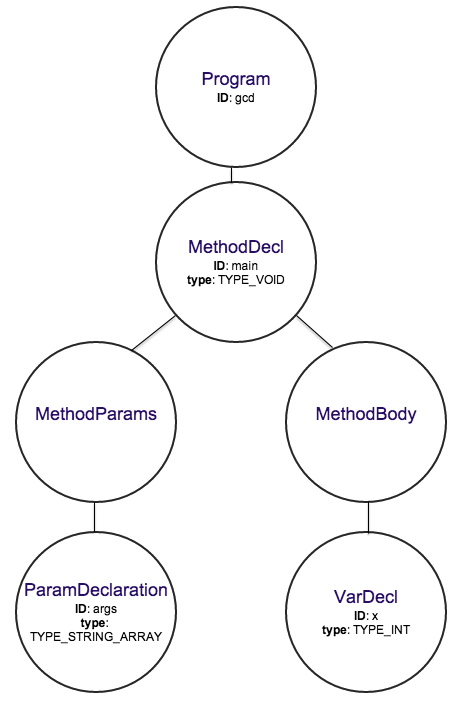
\includegraphics[keepaspectratio=true, scale = 0.5]{arvore.png}
       \caption{Árvore de Sintaxe Abstrata para o Programa Exemplo}
\end{figure}

 

\subsection{Análise Semântica}
A Análise Semântica tem como principais objectivos a ligação das definições de variáveis com a sua utilização, a verificação da correcção de tipos, declarações e chamadas de funções.
Esta análise é dividida em duas fases:
\begin{enumerate}
	\item Para cada \emph{scope no programa:}
	\begin{itemize}
		\item Processar as declarações:
		\begin{itemize}
			\item Adicionar novas entradas na tabela de símbolos
			\item Apresentar mensagem de erro caso haja variáveis repetidas
		\end{itemize}
		\item Processar os \emph{statements}
		\begin{itemize}
			\item Procurar variáveis que não foram declaradas neste \emph{scope} ou no \emph{scope} global, e caso não tenham sido, apresentar mensagem de erro
		\end{itemize}
	\end{itemize}
	\item Processar todos os \emph{statements} do programa outra vez
	\begin{itemize}
		\item Usar a tabela de símbolos para determinar o tipo de cada expressão e procurar erros de tipo (atribuições, cálculos, contagem e tipos de argumentos correctos,...)
	\end{itemize}
\end{enumerate}

\subsection{Tabela de Símbolos}

Para representação da tabela de símbolos, foram utilizadas as seguintes estruturas:
\lstset{language=C,caption={Estruturas para representação da Tabela de Símbolos},label=Estruturas,frame=single}
\begin{lstlisting}
/* Table Node */
typedef struct _TableNode
{
    //Type of the Node (to identify the type of the node)
    TableType n_type;
    
    //Type of the Struct (Int, Void, String,...)
    Type type;
    
    //ID or list of id's
    listID* id;
    
    //Next node
    struct _TableNode* next;
    
    //If is a param
    char isParam;
}TableNode;

/* Table */
typedef struct _Table{
    TableNode* table;
    struct _Table* next;
}Table;

\end{lstlisting}


\pagebreak
\subsection{Tratamento de Erros Semânticos}
Para o tratamento de erros semânticos utilizamos as seguintes funções:
\lstset{language=C,caption={Funções para tratamento de erros semânticos},label=Estruturas,frame=single}
\begin{lstlisting}
/* Check if global variables have the same name as the Methods:
		- If they have print error message: "Symbol %s already defined" and exit 
*/
void   checkIfExists(char* id, Table* local);
void   checkSemanticErrors(Node* ast, Table* local, Table* main);
void   checkErrors(Node* ast, Table* symbols, Table* main);

/* Check if ID exists:
	- If exists return the Type 
	- If doesn't exist, print error message: "Cannot find symbol %s\n" and exit 
*/
int    checkifIDExists(char* id,TableType type, Table* table, Table* main);
Table* getMethodTable(Table* main, char* methodID);

/* Check if the Literal is valid (decimal / hexadecimal / octal)
	- If it is invalid print error message: "Invalid literal %s\n" and exit
*/
void   validIntLit(char* lit);
void   checkTypes(Node* ast,Table* main);
void   operatorError2Types(int op,int n1, int n2);
void   operatorError1Types(int op,int n1);
void   assignmentError(char* var, int n1, int n2);
void   assignmentErrorArray(char* var, int n1, int n2);
void   setTable(Table * oi);
int    getFunctionType();
void   statementError(int op, int n1,int n2);
void   statementError1oranother(int op, int n1, int n2, int n3);
char*  getFunctionName();
void   getErrorCall(int i,char* name, int n1, int n2);

\end{lstlisting}
\pagebreak
\section{Geração de Código}
	


\end{document}